\chapter{Ταυτότητες και Υπολογισμοί}
\section{Ταυτότητες}
\begin{equation}\label{apx_1}
    \frac{\Vec{x}-\Vec{x}\,'}{|\Vec{x}-\Vec{x}\,'|^3} =  -\vec{\nabla}\left(\frac{1}{|\Vec{x}-\Vec{x}\,'|}\right) = \vec{\nabla}'\left(\frac{1}{|\Vec{x}-\Vec{x}\,'|}\right)
\end{equation}

\begin{equation}\label{apx_2}
    \vec{\nabla}\times\left( f\vec{A} \right) \, = \, \vec{\nabla} f \times \vec{A} + f \vec{\nabla}\times\vec{A}
\end{equation}

\begin{equation}\label{apx_3}
    \vec{\nabla}\times\left(\vec{\nabla}\times\vec{A}\right) \, = \, \vec{\nabla}\left( \nabla\cdot\vec{A} \right) - \vec{\nabla}^2\vec{A}
\end{equation}

\begin{equation}\label{apx_4}
    \vec{\nabla}^2\left(\frac{1}{|\vec{x}-\vec{x}\,'|}\right) \, = \, -4\pi\delta^3(\vec{x}-\vec{x}\,\,')
\end{equation}

\begin{equation}
    \nabla\subscr{\lambda} V\superscr{\rho}\,\equiv\,\partial\subscr{\lambda} V\superscr{\rho}\,+\,\con{\rho}{\lambda}{\sigma} V\superscr{\sigma}
\end{equation}
\begin{equation}
    \nabla\subscr{\lambda} T\superscr{\rho}\subscr{\;\;\mu\nu} \,\equiv\,\partial\subscr{\lambda} T\superscr{\rho}\subscr{\;\;\mu\nu}\,+\,\con{\rho}{\lambda}{\sigma}T\superscr{\sigma}\subscr{\;\;\mu\nu} \,-\, \con{\sigma}{\lambda}{\mu}T\superscr{\rho}\subscr{\;\;\sigma\nu} \,-\, \con{\sigma}{\lambda}{\nu}T\superscr{\rho}\subscr{\;\;\mu\sigma}
\end{equation}

\begin{equation}\label{gamma matrix commutator}
    \frac{i}{4}[\gamma\superscr{\mu},\gamma\superscr{\nu}]=S\superscr{\mu\nu}
\end{equation}
\begin{equation}\label{gamma matrix anticommutator}
    \{\gamma\superscr{\mu},\gamma\superscr{\nu}\}=2g\superscr{\mu\nu}\mathbf{1}
\end{equation}

\newpage
\section{Αποδείξεις πράξεων}
\subsection{Όρος μονοπόλου στη συνάρτηση μαγνητικού πεδίου}
\begin{equation}\label{apx_5}
    \int\limits_L\vec{\nabla}\cdot\left(\frac{d\Vec{\ell}'}{|\Vec{x}-\Vec{x}\,'|}\right) = \int\limits_L\vec{\nabla}\left(\frac{1}{|\Vec{x}-\Vec{x}\,'|}\right)\cdot d\Vec{\ell}' = - \int\limits_L\vec{\nabla}'\left(\frac{1}{|\Vec{x}-\Vec{x}\,'|}\right)\cdot d\Vec{x}\,' = - \frac{1}{|\vec{x}-\vec{x}\,'|}
\end{equation}
\begin{note}[\ref{apx_5}]
    Στην τρίτη ισότητα έγιναν οι αντικατάστασεις $d\vec{\ell'} \rightarrow d\vec{x}\,'$ και $\vec{\nabla}\rightarrow-\vec{\nabla}'$ (ταυτότητα \eqref{apx_1}). Το απειροστό μήκος $d\vec{\ell'}$ στην επικαμπύλια ολοκλήρωση ισούται με την απειροστή μετατόπιση %διαφορικό μήκος στο σύστημα 
    $d\vec{x}\,'$, κατά μήκος της χορδής Dirac.
\end{note}

\subsection{Διαφορά δυναμικού μεταξύ δύο χορδών Dirac}\label{apx22}
\begin{theorem}[Stokes]
\begin{equation}\label{stokes}
    \qquad\oint\limits\subscr{C=\partial S} \vec{F} \, \cdot \,d\vec{\ell} = \iint\limits\subscr{S}\left(\vec{\nabla}\times\vec{F}\right)\cdot d\superscr{2}\vec{x}
\end{equation}    
\end{theorem}

Έστω η διανυσματική συνάρτηση $\vec{F} = \scafun{f}{\vec{x}}\,\vec{g}$, όπου $\vec{g}$ ανεξάρτητο του $\vec{x}$:
\begin{align}
    \oint\limits\subscr{C} \scafun{f}{\vec{x}}\,\vec{g}\cdot d\vec{\ell}\, & = \, \iint\subscr{S}\left(\,\vec{\nabla}\times (\scafun{f}{\vec{x}}\vec{g})\,\right)\cdot d\superscr{2}\vec{x}\label{stokes1}\\
    \vec{g}\cdot \oint \scafun{f}{\vec{x}} d\vec{\ell} \, &= \, \iint\subscr{S}\left(\vec{\nabla} f \times\vec{g}\,+\,\cancelto{\text{\scalebox{0.7}{0}}}{f(\vec{\nabla}\times\vec{g})}\quad\right)\cdot d\superscr{2}\vec{x} \label{stokes2}\\
    &= \, -\,\vec{g}\cdot\iint\subscr{S}\vec{\nabla} f \times d\superscr{2}\vec{x} \label{stokes3}\\
    \Rightarrow \oint \scafun{f}{\,\vec{x}\,\,} d\vec{\ell} \, &= \, -\, \iint\subscr{S} \nabla f \times d\superscr{2}\vec{x}\label{stokes4}\\
    \Rightarrow \oint \scafun{f}{|\,\vec{x}-\vec{x}\,'\,|}\,\,d\vec{\ell}' \, &= \, -\,\iint\subscr{S}\vec{\nabla} ' f \times d\superscr{2}\vec{x}\,' \, = \, \,\iint\subscr{S}\vec{\nabla} f \times d\superscr{2}\vec{x}\,' \label{stokes5}
\end{align}



\begin{note}[\ref{stokes1}-\ref{stokes4}]
    Στην \eqref{stokes2} χρησιμοποιήσαμε την \eqref{apx_2}. Η μετάθεση των διανυσμάτων της \eqref{stokes3} έγινε ως εξής 
    \begin{align*}
        \left(\vec{\nabla} f \times \vec{g}\right)\cdot d \vec{A} &= \, \epsilon^{ijk} \left( \vec{\nabla} f \right)^j g^k\left( d\vec{A}\right)^i \, = \, -\epsilon^{ijk} \left( \vec{\nabla} f \right)^j \left( d\vec{A}\right)^k g^i = -\vec{g}\cdot\left(\vec{\nabla} f \times d\vec{A}\right)
    \end{align*}
\end{note}

\newpage

\subsection{Δύο χορδές Dirac}\label{apx23}
Ακολούθως εφαρμόζουμε το αποτελέσμα \eqref{vecpotdif3} για δύο χορδές Dirac, όπως φαίνονται στο σχήμα \ref{fig:solidangle}. Αρκεί να εξεταστούν οι δύο αυτές διαμορφώσεις, για να γίνει εμφανές η συνάρτηση $\scafun{\Omega}{\vec{x}}$ της \eqref{vecpotdif3} είναι πλειότιμη, που όμως σε συνδυασμό με τον δεύτερο όρο δίνουν την καλά ορισμένη διαφορά δυναμικών $ \vecfun[L']{A}{\vec{x}} - \vecfun[L]{A}{\vec{x}}$.

\begin{figure}[h]
    \centering
    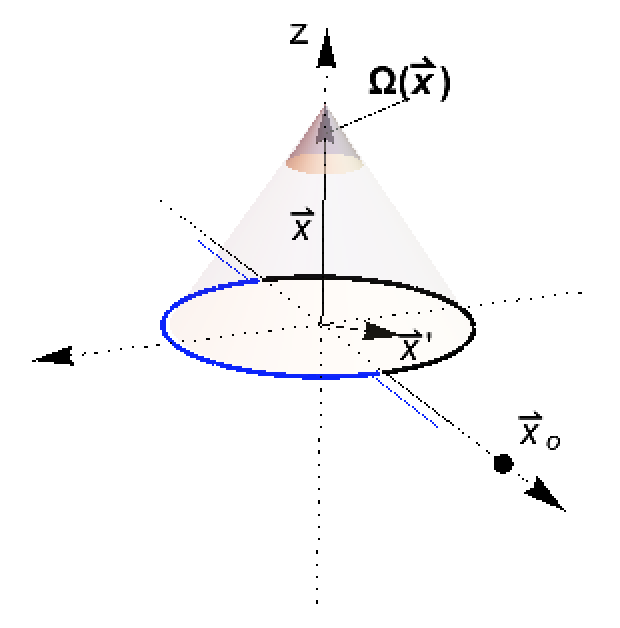
\includegraphics[width=7cm, height=7cm]{solid angle.png}
    \caption{\textit{Δύο ημιάπειρες χορδές Dirac. Οι χορδές τρέχουν παράλληλα κατά μήκος ενός άξονα, σε απειροστά μικρή απόσταση μεταξύ τους, και στη συνέχεια κατά μήκος αντιδιαμετρικών ημικυκλίων ακτίνας $R '$ και κέντρο την αρχή των αξόνων. Κάθε χορδή τερματίζεται στο σημείο $\vec{x}_0$. %αλληλοεπικαλύπτονται σχεδόν παντού και είναι παράλληλες με %ένα κύριο άξονα. Η τοποθέτησή τους περιέχει ημικυκλικό %τομέα με ακτίνα $R '$ ως προς την αρχή των αξόνων. Οι δύο %τομείς είναι στο ίδιο επίπεδο (x-y) αλλά δεν %αλληλοεπικαλύπτονται. Η χορδή τερματίζει στο σημείο 
    }}
    \label{fig:solidangle}
\end{figure}

Εκτελούμε το πρώτο επιφανειακό ολοκλήρωμα της \eqref{vecpotdif3} πραγατοποιώντας το πρώτο. Η επιφάνεια $S$ είναι ο δίσκος
\begin{equation*}
    \pvec{x}' = \big\{ \, (x',\y',0)\quad|\quad \sqrt{x'^2+\y'^2}\le R \, \big\} \quad \forall \, \pvec{x}'\in S
\end{equation*}
Σε πολικές συντεταγμένες έχουμε $\pvec{x}' = \rho'\hat{\rho}'$, %το διαφορικό στοιχείο επιφάνειας 
$d\pvec{s}' = \rho' d\rho' d\phi' \hat{z}$ και το σημείο παρατήρησης είναι το $\vec{x} = \rho\hat{\rho}+z\hat{z}$. Για χάριν απλότητας επιλέγουμε το σημείο παρατήρησης στον άξονα $z$ ($\rho = 0$) και παίρνουμε
\begin{equation}\label{apx_solidangle1}
    \scafun{\Omega}{\vec{x}} \,=\, \int\limits_0^{R}\int\limits_0^{2\pi} \frac{\rho'\hat{\rho}'-z\hat{z}}{\left(z^2+\rho'^2\right)^{3/2}}\cdot \rho'd\rho'd\phi'\hat{z} \,=\, -\int\limits_0^{R}\int\limits_0^{2\pi}\frac{z\,\rho'd\rho'd\phi'}{\left(z^2+\rho'^2\right)^{3/2}}
\end{equation}
\\

Με προσεκτική διερεύνηση, μπορούμε να διακρίνουμε την πλειοτιμία της \eqref{apx_solidangle1}. Στο όριο που προσεγγίζουμε την επιφάνεια από τον θετικό άξονα z ($z\rightarrow 0^+$), παίρνουμε\footnote{Για τη δεύτερη ισότητα έγινε η αντικατάσταση $\rho'\rightarrow\frac{\rho'}{|z|}$.}
\begin{equation}\label{apx_solidangle2}
    \scafun{\Omega}{\vec{x}}\,=\,-\lim\limits_{z\rightarrow 0^+}2\pi\int\limits_0^{R}\frac{z\,\rho'd\rho'}{\left(z^2+\rho'^2\right)^{3/2}} \,=\, -\lim\limits_{z\rightarrow 0^+}2\pi\int\limits_0^{R/z}\frac{\rho'd\rho'}{\left(1+\rho'^2\right)^{3/2}} \,=\, -2\pi
\end{equation}
Στο όριο που προσεγγίζουμε την επιφάνεια από τον αρνητικό άξονα των $z$ ($z\rightarrow 0^-$), παίρνουμε\footnote{Επειδή το $z$ είναι αρνητικό, ο αριθμητής είναι θετικός.} 
%πρέπει να χειριστούμε με σύνεση το αρνητικό πρόσιμο που φέρει %το z στον αριθμητή. Η \eqref{apx_solidangle1} μας δίνει τώρα
\begin{equation}\label{apx_solidangle3}
    \scafun{\Omega}{\vec{x}}\,=\, \lim\limits_{z\rightarrow 0^-}2\pi\int\limits_0^{R/z}\frac{\rho'd\rho'}{\left(1+\rho'^2\right)^{3/2}} \,=\, +2\pi
\end{equation}

Τα αποτελέσματα \eqref{apx_solidangle2} και \eqref{apx_solidangle3} είναι ανεξάρτητα της ακτίνας και του επιπέδου στο οποίο βρίσκεται ο δίσκος. 
%του συνόρου και του προσανατολισμού της επίπεδης επιφάνειας %S\footnote{Η αποδοχή του πιο πάνω είναι εύκολη διαισθητικά %αφού, ως προς ένα σημείο μάνω σε κάποια επίπεδη επιφάνεια, η %γωνία που πρέπει να καλύψουμε ακολουθώντας  ολόκληρο το κλειστό %σύνορο της επιφάνειας είναι $2\pi$ . Από που πλησιάζουμε το %σημείο αυτό της επιφάνειας καθορίζει και το πρόσιμο της στερεάς %γωνίας}. 
Συνοψίζοντας, έχουμε τα ακόλουθα
\begin{equation*}
    \scafun{\Omega}{\vec{x}} \,\rightarrow\, \left\{\begin{array}{cc} -2\pi & z \rightarrow 0^+\\ 2\pi & z\rightarrow0^-
            \end{array} \right. 
\end{equation*}
Διαμέσου της επιφάνειας $S$ του σχήματος \ref{fig:solidangle} ($\vec{x}\rightarrow\pvec{x}'\in S$) η συνάρτηση $\scafun{\Omega}{\vec{x}}$ αλλάζει πρόσημο. Έτσι, η κλίση της είναι 
\begin{equation}\label{derivsolidangle}
    \lim\limits_{\vec{x}\rightarrow\pvec{x}'\in S} \vec{\nabla} \Omega(\vec{x}) = -4\pi \, \scafun{\delta}{z}\hat{z}
\end{equation}
\\
O δεύτερος όρος της \eqref{vecpotdif3} υπολογίζεται ως εξής
\begin{equation}\label{apx_deltaint}
    \int\limits_S  \scafun{\delta}{\vec{x}-\pvec{x}'} d\pvec{s}' \,=\, \int\limits_0^R\int\limits_0^{2\pi}\scafun{\delta}{z\hat{z}-\rho'\hat{\rho}'}\rho'd\rho'd\phi'\hat{z} = \int\limits_0^R\int\limits_0^{2\pi}\frac{\scafun{\delta}{z}\scafun{\delta}{\rho'}}{2\pi\rho'}\rho'd\rho'd\phi'\hat{z} = \scafun{\delta}{z}\hat{z}
\end{equation}
Αντικαθιστώντας τις \eqref{derivsolidangle} και \eqref{apx_deltaint} στην \eqref{vecpotdif3}, συμπεραίνουμε ότι η διαφορά \eqref{vecpotdif3} είναι καλά ορισμένη. 


\subsection{Μεταβολή δράσης Eistein-Hilbert}\label{EHvar}

\begin{equation}
    \delta\R[\rho]{\mu}[\lambda]{\nu} \,=\, \partial\subscr{\lambda}\delta\Gamma\superscr{\rho}\subscr{\;\;\mu\nu} \,+\, \delta\Gamma\superscr{\rho}\subscr{\;\;\lambda\sigma}\Gamma\superscr{\sigma}\subscr{\;\;\mu\nu} \,+\, \Gamma\superscr{\rho}\subscr{\;\;\lambda\sigma}\delta\Gamma\superscr{\sigma}\subscr{\;\;\mu\nu} \,-\, \partial\subscr{\nu}\delta\Gamma\superscr{\rho}\subscr{\;\;\mu\lambda} \,-\, \delta\Gamma\superscr{\rho}\subscr{\;\;\nu\sigma}\Gamma\superscr{\sigma}\subscr{\;\;\mu\lambda} \,-\, \Gamma\superscr{\rho}\subscr{\;\;\nu\sigma}\delta\Gamma\superscr{\sigma}\subscr{\;\;\mu\lambda}
\end{equation}
\begin{equation}
    \nabla\subscr{\lambda}\left(\delta\con{\rho}{\mu}{\nu}\right) \,=\, \partial\subscr{\lambda}\delta\Gamma\superscr{\rho}\subscr{\;\;\mu\nu} \,+\, \Gamma\superscr{\rho}\subscr{\;\;\sigma\lambda}\delta\Gamma\superscr{\sigma}\subscr{\;\;\mu\nu} \,-\, \Gamma\superscr{\sigma}\subscr{\;\;\nu\lambda}\delta\Gamma\superscr{\rho}\subscr{\;\;\mu\sigma} \,-\, \con{\sigma}{\mu}{\lambda}\delta\con{\rho}{\nu}{\sigma}
\end{equation}
\begin{equation}
    \nabla\subscr{\nu}\left(\delta\con{\rho}{\mu}{\lambda}\right) \,=\, \partial\subscr{\nu}\delta\con{\rho}{\mu}{\lambda} \,+\, \con{\rho}{\sigma}{\nu}\delta\con{\sigma}{\mu}{\lambda} \,-\, \con{\sigma}{\lambda}{\nu}\delta\con{\rho}{\mu}{\sigma} \,-\, \con{\sigma}{\mu}{\nu}\delta\con{\rho}{\sigma}{\lambda}
\end{equation}
\begin{equation}
    \delta\R[\rho]{\mu}[\lambda]{\nu} \,=\, \nabla\subscr{\lambda}\delta\con{\rho}{\mu}{\nu} \,-\, \nabla\subscr{\nu}\delta\con{\rho}{\mu}{\lambda}
\end{equation}
\begin{equation}
    \delta\R{\mu}{\nu} \,=\, \delta\R[\lambda]{\mu}[\lambda]{\nu} \,=\, \nabla\subscr{\lambda}\delta\con{\lambda}{\mu}{\nu} \,-\, \nabla\subscr{\nu}\delta\con{\lambda}{\mu}{\lambda}
\end{equation}
\begin{equation}
\begin{split}
    \int \sqrt{-g} \,\g[i]{\mu}{\nu}\,\delta\R{\mu}{\nu}\,d\superscr{4}x \,&=\, \int \sqrt{-g} \,\g[i]{\mu}{\nu} \,\left( \nabla\subscr{\lambda}\delta\con{\lambda}{\mu}{\nu} \,-\, \nabla\subscr{\nu}\delta\con{\lambda}{\mu}{\lambda} \right)\,d\superscr{4}x\\
    &=\, \int\,\sqrt{-g}\left( \nabla\subscr{\lambda}\left(\g[i]{\mu}{\nu}\delta\con{\lambda}{\mu}{\nu}\right) \,-\, \nabla\subscr{\nu}\left(\g[i]{\mu}{\nu}\delta\con{\lambda}{\mu}{\lambda}\right) \right)\,d\superscr{4}x\\
    &=\, \int\,\sqrt{-g}\,\nabla\subscr{\nu}\left(\g[i]{\mu}{\lambda}\delta\con{\nu}{\mu}{\lambda} \,-\,\g[i]{\mu}{\nu}\delta\con{\lambda}{\mu}{\lambda} \right)\,d\superscr{4}x\\
    &=\, 0
    \end{split}
\end{equation}

\subsection{Μεταβολή δράσης Maxwell}\label{Maxwvar}
%Τα σύμβολα ολοκλήρωσης $\int d\superscr{4}x$ αγνοήθηκαν λόγω $συνωστισμού
\begin{equation}
\begin{split}
    \de\subscr{g} L\subscr{M}&=-\frac{1}{4}F\subscr{\mu\nu}F\subscr{\alpha\beta}\left( \de\g[1]{\mu}{\alpha}\g[1]{\nu}{\beta} \,+\, \g[1]{\mu}{\alpha}\de\g[1]{\nu}{\beta} \right)\sqrt{-g}\,\,-\,\,\frac{1}{4}F\superscr{2}\de\sqrt{-g}\\
    &=-\frac{1}{4}\left(F\subscr{\mu\nu}F\subscr{\alpha\beta} \de\g[1]{\mu}{\alpha}\g[1]{\nu}{\beta} \,+\, F\subscr{\nu\mu}F\subscr{\beta\alpha}\g[1]{\nu}{\beta}\de\g[1]{\mu}{\alpha} \right)\sqrt{-g}\,\,-\,\,\frac{1}{4}F\superscr{2}(-\frac{1}{2}\sqrt{-g}\g{\mu}{\alpha}\de\g[1]{\mu}{\alpha})\\
    &=-\left(\frac{1}{2}F\subscr{\mu\nu}F\subscr{\alpha\beta} \de\g[1]{\mu}{\alpha}\g[1]{\nu}{\beta}\,\,-\,\,\frac{1}{8}F\superscr{2}\g{\mu}{alpha}\right)\sqrt{-g}\de\g[1]{\mu}{\alpha}
\end{split}
\end{equation}

\section{Λύση διαφορικής εξίσωσης \ref{differential equation for metric components}}\label{solution for metric dif eq}
Η διαφορική εξίσωση πρώτου βαθμού είναι γραμμική και μη ομογενής. Γράφεται στην ακόλουθη μορφή για τον προσδιορισμό του ολοκληρωτικού παράγοντα 
%(πολλαπλασιαστής Euler) 
$\mu(r)$
\begin{equation}
\begin{split}
    &2r\frac{db}{dr}+e^{2b}(1-\frac{A}{r\superscr{2}})-1=0\\
    &2\frac{db}{dr}e\superscr{-2b}+(\frac{1}{r}-\frac{A}{r\superscr{3}})-\frac{e\superscr{-2b}}{r}=0\\
    &\frac{d}{dr}(e\superscr{-2b})+\frac{e\superscr{-2b}}{r}=\left(\frac{1}{r}-\frac{A}{r\superscr{3}} \right)\\
\end{split}
\end{equation}
Με την αντικατάσταση $\y\equiv e\superscr{-2b}$ 
\begin{equation}\label{inappendix reference differential equation}
    \y'+\frac{1}{r}\y - \left(\frac{1}{r}-\frac{A}{r\superscr{3}} \right) = 0
\end{equation}
η εξίσωση παίρνει τη μορφή 
\begin{equation}
    N(r,\y)\y' + M(r,\y)=0
\end{equation}
επιτρέποντας τον προσδιορισμό του $\mu(r)$
\begin{equation}
    \mu(r) = \exp\left( \int \frac{M\subscr{\y}-N\subscr{r}}{N} \right) = \exp\left( \int \frac{1}{r} dr \right) = r
\end{equation}
Πολλαπλασιάζοντας τώρα την \eqref{inappendix reference differential equation} με $\mu$, η δ.ε. γίνεται
\begin{equation}
    \frac{d}{dr}(\mu y) = \mu \left( \frac{1}{r}-\frac{A}{r\superscr{3}} \right)
\end{equation}
η λύση της οποίας είναι επίσης λύση της \eqref{inappendix reference differential equation}. Oλοκληρώνοντας στο διάστημα $[r\subscr{o},r]$ ($r\subscr{o}\ne0$), βρίσκουμε τη γενική λύση 
\begin{equation}
    \y(r) = 1+\frac{A}{r\superscr{2}}-\frac{c(r\subscr{o})}{r}\quad\Rightarrow\quad b(r)=-\frac{1}{2}\ln\left(1+\frac{A}{r\superscr{2}}-\frac{c(r\subscr{o})}{r}\right)
\end{equation}